\documentclass{beamer}

\mode<presentation>
{
  \usetheme{CambridgeUS}
  \usecolortheme{seagull}
  \setbeamercovered{transparent}
}

\usepackage[english]{babel}
\usepackage[latin1]{inputenc}
\usepackage{times}
\usepackage[T1]{fontenc} 
% Or whatever. Note that the encoding and the font should match. If T1
% does not look nice, try deleting the line with the fontenc.
\usepackage{amsmath}

\newcommand{\linespace}{\vskip 0.25cm}

\definecolor{MyForestGreen}{rgb}{0,0.7,0} 
\newcommand{\tableemph}[1]{{#1}}
\newcommand{\tablewin}[1]{\tableemph{#1}}
\newcommand{\tablemid}[1]{\tableemph{#1}}
\newcommand{\tablelose}[1]{\tableemph{#1}}

\definecolor{MyLightGray}{rgb}{0.6,0.6,0.6}
\newcommand{\tabletie}[1]{\color{MyLightGray} {#1}}

% The text in square brackets is the short version of your title and will be used in the
% header/footer depending on your theme.
\title[Concurrent Compaction in JVM GC]{Concurrent Compaction in JVM Garbage Collection}

% Sub-titles are optional - uncomment and edit the next line if you want one.
% \subtitle{Why does sub-tree crossover work?} 

% The text in square brackets is the short version of your name(s) and will be used in the
% header/footer depending on your theme.
\author[Jacob Opdahl]{Jacob P. Opdahl}


% The text in square brackets is the short version of your institution and will be used in the
% header/footer depending on your theme.
\institute[UMM]
{
  University of Minnesota, Morris \\[\baselineskip]
  \emph{opdah023@morris.umn.edu}
}

% The text in square brackets is the short version of the date if you need that.
\date[December 5, 2015] % (optional)
{December 5, 2015}

% Delete this, if you do not want the table of contents to pop up at
% the beginning of each subsection:
%\AtBeginSection[]
%{
%  \begin{frame}<beamer>
%    \frametitle{Outline}
%    \tableofcontents[currentsection, hideothersubsections]
%  \end{frame}
%}

\begin{document}

\begin{frame}
  \titlepage
\end{frame}

% For a 20-25 minute senior seminar talk you probably want something like:
% - Two or three major sections (other than the summary).
% - At *most* three subsections per section.
% - Talk about 30s to 2min per frame. So there should probably be between
%   15 and 30 frames, all told.



\section*{Overview}

\subsection*{Garbage Collection}

%\begin{frame}
%\end{frame}



\subsection*{Outline}

\begin{frame}
  \frametitle{Outline}
  \tableofcontents  
  %\tableofcontents[hidesubsections]
\end{frame}



\section[Introduction]{Introduction}

\subsection[GC Basics]{Garbage Collection Basics}



\subsection[PP Basics]{Parallel Processing Basics}



\subsection[GC with PP]{Garbage Collection with Parallel Processing}



\section[C4]{Continuously Concurrent Compacting Collector (C4)}

\subsection*{Explanation}



\subsection*{Test Results}



\section[Collie]{Collie Collector}

\subsection*{Explanation}



\subsection*{Test Results}



\section[FPP]{Field Pinning Protocol}

\subsection*{Explanation}

\begin{frame}

\frametitle{The Blame Game}

\only<1>{

\begin{itemize}
\item \emph{blamed} thread: responsible for relocating an object

\begin{itemize}
\item Comes from HPs interrupting copying
\end{itemize}
\end{itemize}

\linespace
\linespace

\begin{enumerate}
\item GC threads attempt to relocate objects
\begin{itemize}
\item No blame passed!
\end{itemize}

\item GC threads try again... blame if interrupted
\item Blame continues to be passed to interrupting threads
\end{enumerate}

} %End only<1>

\only<2>{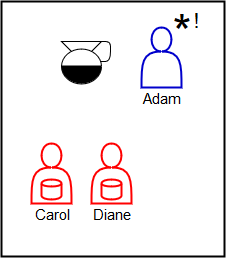
\includegraphics[width=.95\textwidth]{Illustrations/coffeeLine1.png}}
\only<3>{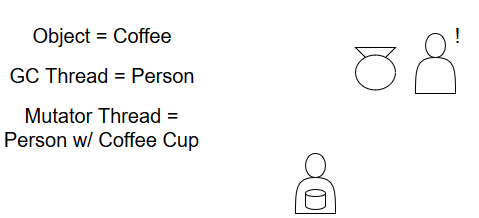
\includegraphics[width=.95\textwidth]{Illustrations/coffeeLine2.png}}
\only<4>{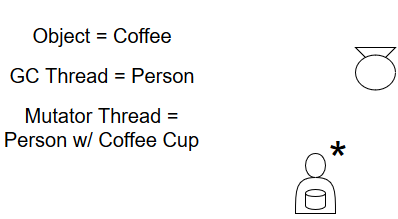
\includegraphics[width=.95\textwidth]{Illustrations/coffeeLine3.png}}
\only<5>{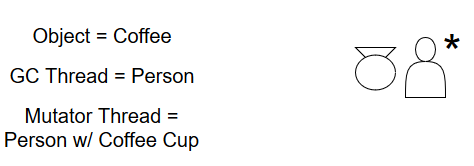
\includegraphics[width=.95\textwidth]{Illustrations/coffeeLine4.png}}
\only<6>{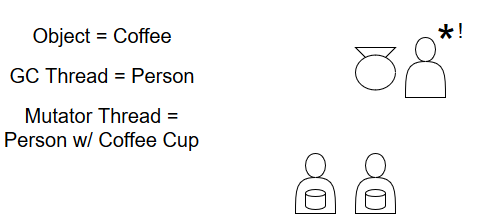
\includegraphics[width=.95\textwidth]{Illustrations/coffeeLine5.png}}

\end{frame}


\subsection*{Test Results}



\section[Conclusions]{Conclusions}

\begin{frame}
	\frametitle{Thanks for your time!}
	
	\begin{center}
	{\huge Questions?}
	\end{center}	
	
	\linespace
	\linespace	
	
	\begin{center}
	Contact: opdah023@morris.umn.edu
	\end{center}
	
\end{frame}



\section*{References}

\begin{frame} 
	\frametitle{References} 
	
%	\begin{thebibliography}{lskdjf}
%	
%	\bibitem{McPhee:2009:gecco}
%N.~F. McPhee, E.~Crane, S.~Lahr, and R.~Poli.
%\newblock Developmental Plasticity in Linear Genetic Programming.
%\newblock In G\"unther Raidl, \emph{et al}, editors, {\em GECCO '09}, pages 1019--1026, Montr\'eal, Qu\'ebec, Canada, 2009.
%	
%	\bibitem{citeulike:3452411}
%	R.~Poli and N.~McPhee.
%\newblock A linear estimation-of-distribution {GP} system.
%\newblock In M.~O'Neill, \emph{et al}, editors, {\em EuroGP 2008}, volume
%  4971 of {\em LNCS}, pages 206--217, Naples,
%  26-28 Mar. 2008. Springer.
%  
%  	\end{thebibliography}
%	
%	\linespace
%	\begin{center}
%	See the GECCO '09 paper for additional references.
%	\end{center}
\end{frame} 



\end{document}


